\chapter{Padrões Estruturais}

\section{Adapter}

Quando a interface de uma classe não 
é compatível com a interface do cliente que deseja 
utilizá-la, o padrão Adapter fornece uma 
solução que evita a refatoração e a dependência da 
interface do cliente com a interface desejada.\cite{gamma:1995}

Existem duas formas de realizar essa adaptação. Um Adapter 
de classe, apresentado na figura \ref{adapter_struct},  
só é possível para linguagens que implementam herança 
múltipla.
Ele define uma classe que herda tanto da classe que 
apresenta a interface do cliente quanto da classe que 
apresenta a interface que deseja ser utilizada. Ao 
reescrever a operação Request, ele adapta sua entrada 
para a de SpecificRequest, repassando a solicitação.\cite{gamma:1995}

\begin{figure}[htb]
	\caption{\label{adapter_struct}Estrutura do Adapter de Classe}
	\begin{center}
	    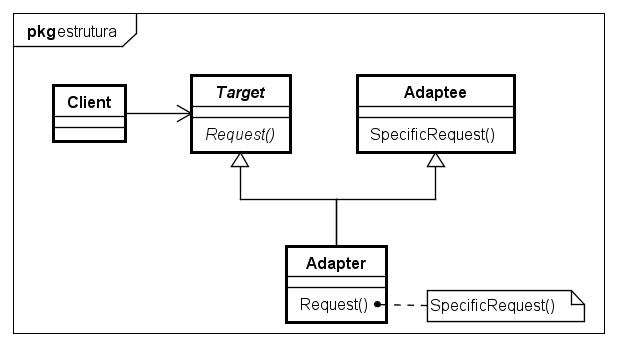
\includegraphics[scale=0.5]{5_padroes-contexto-funcional/5.2_estruturais/5.2.1_adapter/adapter_classe_estrutura.png}
	\end{center}
\end{figure}

Já o Adapter de Objeto, apresentado na figura \ref{adapter_alt_struct}, 
herda apenas da classe que apresenta a interface 
da aplicação, também reimplementando a operação Request. 
A diferença é que ela repassa a solicitação para a 
classe que apresenta a interface que deseja ser 
utilizada através de uma delegação.\cite{gamma:1995}

\begin{figure}[htb]
	\caption{\label{adapter_alt_struct}Estrutura do Adapter de Objeto}
	\begin{center}
	    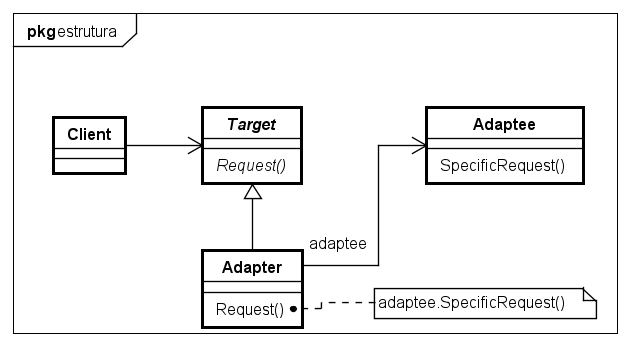
\includegraphics[scale=0.5]{5_padroes-contexto-funcional/5.2_estruturais/5.2.1_adapter/adapter_objeto_estrutura.png}
	\end{center}
\end{figure}

\subsection*{Exemplo Orientado a Objetos}

Como exemplo é apresentada uma ferramenta gráfica 
que permite a edição de diversos objetos gráficos 
simples, entre eles linhas e polígonos. Porém, 
a aplicação deseja também editar elementos textuais, 
que são mais complexos de se gerenciar. Como já existem 
ferramentas prontas para gerenciar esse tipo de 
elemento, é desejado reutilizá-las. Como essas 
ferramentas não foram feitas pensando na 
aplicação de ferramenta gráfica do exemplo, uma 
classe Adapter é implementada para adaptar a 
ferramenta textual para a aplicação que deseja 
utilizá-la. Para esse exemplo, é utilizada a 
abordagem de Adapter de objeto, onde um objeto 
do tipo da ferramenta textual é armazenado. O 
diagrama de classes do exemplo pode ser visto na 
figura \ref{adapter_exemplo}, enquanto a 
implementação em código pode ser vista no código 
\ref{ooadapter}.


\begin{figure}[htb]
	\caption{\label{adapter_exemplo}Exemplo de Adapter}
	\begin{center}
	    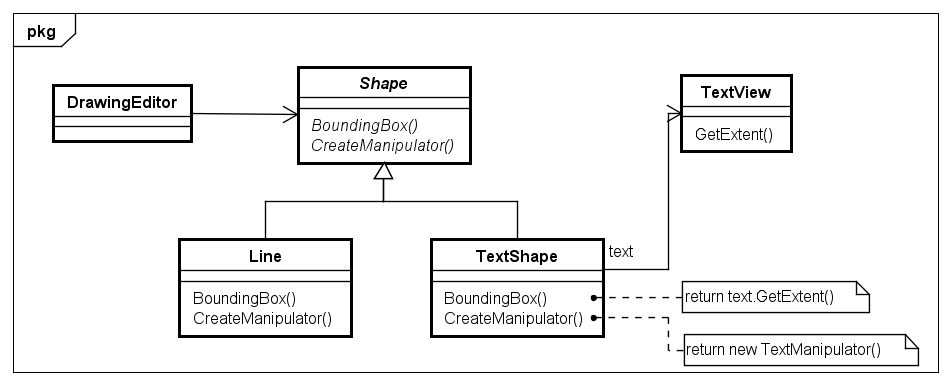
\includegraphics[scale=0.5]{5_padroes-contexto-funcional/5.2_estruturais/5.2.1_adapter/adapter_exemplo.png}
	\end{center}
\end{figure}


\begin{lstlisting}[caption={Adapter Orientado a Objetos},label=ooadapter]

class DrawingEditor(shape : Shape) {

}

abstract class Shape(var bottomLeft : Point, var topRight : Point) {
  def BoundingBox() : Int
  def CreateManipulator()
}

class Line(bottomLeft : Point, topRight : Point)
  extends Shape(bottomLeft, topRight) {

  def BoundingBox() : Int = 0
  def CreateManipulator() : Unit = {
    //Line Manipulator
  }
}

class TextShape(bottomLeft : Point, topRight : Point, text : TextView)
  extends Shape(bottomLeft, topRight) {

  def BoundingBox() : Int = text.GetExtent()
  def CreateManipulator() : Unit = {
    //TextManipulator
  }
}

class TextView(var x : Point, var y : Point, var width : Int, var height : Int) {
  def GetExtent() : Int = {
    // Retorna extensão do texto
  }
}

\end{lstlisting}

\subsection*{Contexto Funcional}

No código \ref{fpadapter}, a função DrawingEditorFunction 
declarada na linha 2 recebe como parâmetro uma operação de um 
objeto gráfico. Porém, é desejado utilizar a operação 
GetExtent, declarada na linha 7, de um \textit{text view} 
que não é comportado pela ferramenta. Para que essa 
operação possa ser reutilizada, a função 
AdaptTextShapeBoundingBox declarada na linha 11 
recebe como parâmetro o \textit{text view} e retorna 
uma função que executa GetExtent, com a assinatura 
necessária para ser recebida pela função 
DrawingEditorFunction. Com o uso das funções de alta 
ordem, foi necessário apenas uma nova função intermediária 
para realizar a adaptação. 

\begin{lstlisting}[caption={Adapter Funcional},label=fpadapter]
    
def DrawingEditorFunction(CalculateBounding : () => Int) : Int = {
  // ...
  CalculateBounding()
}

def GetExtent(view : TextView) : Int = {
  //Retorna extensão do texto
}

def AdaptTextShapeBoundingBox(view : TextView): () => Int =
  () => {
    // ...
    GetExtent(view)
  }

\end{lstlisting}
